\documentclass[11pt]{article}
\usepackage{matt}
\begin{document}

\section*{Update for the Week of \today}


\begin{figure}[h]
  \centering
  \includegraphics[width=20cm]{gridPlot.png}
  \caption{After adjusting precisely how we weight stacking contributions from different spectra, we show the results of stacking with different thresholds for what constitutes saturated absorption ($\tilde{\sigma}_{\text{N}}$ (top row), $3\tilde{\sigma_{\text{N}}}$ (middle), and $5\tilde{\sigma}_{\text{N}}$ (bottom row)). We also vary the minimum redshift of a pixel for a corresponding dark gap to be included between the different columns. We consider dark gaps with $L_{\text{gap}} < 300\ \kms$ (dashed), $L_{\text{gap}} > 100\ \kms$, 300 \kms, 500 \kms, 1000 \kms.}
  \label{fig:grid}
\end{figure}

\begin{figure}[h]
  \centering
  \includegraphics[width=20cm]{gridPlot_noZ599.png}
  \caption{This figure is the same as Figure \ref{fig:grid} except that we have excluded one spectrum that was contributing significantly more stacks than the others.}
  \label{fig:regrid}
\end{figure}

\begin{figure}[h]
  \centering
  \includegraphics[width=20cm]{gridPlot_UseLyb.png}
  \caption{This figure is the same as Figure \ref{fig:grid} except that we have stacked \lya\ transmission based on dark gaps in \lyb.}
  \label{fig:regrid}
\end{figure}

\begin{figure}[h]
  \centering
  \includegraphics[width=20cm]{gridPlot_noZ599_UseLyb.png}
  \caption{This figure is the same as Figure \ref{fig:grid} except that we have stacked \lya\ transmission based on dark gaps in \lyb\ and excluded one spectrum that was contributing significantly more stacks than the others.}
  \label{fig:regrid}
\end{figure}

\begin{figure}[h]
  \centering
  \includegraphics[width=8cm]{NewWeighting_ErrorBars.png}
  \caption{The above figure shows a stack of the transmission outside of small dark gaps (dashed red) and large dark gaps (solid) with error bars corresponding to $\frac{1}{\sigma_{\mu}^{2}} = \sum_i \frac{1}{\bar{\alpha} \sigma_{\text{N,red}}^{2} + \sigma_{\text{F}}^{2}}$. }
  \label{fig:todo}
\end{figure}


\begin{figure}[h]
  \centering
  %\includegraphics[width=8cm]{WeightingDist.png}
  \includegraphics[width=8cm]{CountsVsZ.png}
  \includegraphics[width=8cm]{WeightingVsZ.png}
  \caption{The left-hand figure shows the distribution of weightings for the individual contributions to the stacks. The right-hand figure shows the number of stacks contributed to the overall average from each spectrum as a function of the spectrum's redshift. This suggests that a spectrum near $z \approx 6$ may be dominating the stack. We re-generate Figure \ref{fig:grid} after excluding this spectrum to obtain Figure \ref{fig:regrid}.}
  \label{fig:todo}
\end{figure}

\begin{figure}[h]
  \centering
  \includegraphics[width=8cm]{NcontributionsVsZ_1200min.png}
  \includegraphics[width=8cm]{ThresholdVsZ_1200min.png}
  \caption{The left-hand figure shows the number of stacks that each spectra contributed as a function of the redshift of the spectrum. This is done only for $L_{\text{dark}} > 1200\ \kms$. The right-hand figure shows the threshold for which a pixel in smoothed spectrum is consistent with saturated absorption, let's call it $f_{\text{thresh}} \equiv t \tilde{\sigma}_{N}$, where we have been using $t = 3$. Together, these \textit{could be} consistent with the idea that large initial stacked transmission is due to large threshold transmissions for a pixel to no longer be consistent with saturated absorption. If this was the case, we would expect the initial stacked transmission to be $\bar{f}_{\text{initial}} \approx \dfrac{1}{\sum N_i w_i} \sum_{i} N_{\text{contributions,i}} w_{i} f_{\text{thresh},i}$. We evaluate this weighted average for $L_{\text{min}} = 1000\ \kms$ and find $\bar{f}_{\text{initial,guess}} = 0.26$. This should be compared to the largest-$L$ curve in the middle-left panel of Figure \ref{fig:grid}. Repeating estimates with other $L_{\text{min}}$, we find $f_{\text{initial,guess}} \approx 0.21$, and 0.16 for $L_{\text{min}} = 500\ \kms$ and 300\ \kms, respectively. The same number for $z_{\text{min}} = 5.5$ are $f_{\text{initial,guess}} \approx $ .1, .07, and .07. }
  \label{fig:todo}
\end{figure}

%
%\begin{figure}[h]
%  \centering
%  \includegraphics[width=8cm]{NaiveWeightingDistribution.png}
%  \includegraphics[width=8cm]{NaiveStack.png}
%  \includegraphics[width=8cm]{EstimatedVarianceWeightingDistribution.png}
%  \includegraphics[width=8cm]{EstimatedVarianceStack.png}
%  \includegraphics[width=8cm]{FluxVarianceWeightingDistribution.png}
%  \includegraphics[width=8cm]{FluxVarianceStack.png}
%  \caption{Results of various spectra-weighting schemes. The left-hand panels show the relative weightings of each contribution to the quasar spectra stacks while the right-hand figures show the resulting stack. The first row uses a basic inverse-variance weighting, the second row does the same but estimates the variance from a segment redward of \lya, and the third row uses an inverse variance weighting where the variance is just the overall variance of the transmission in the spectra. In the basic inverse-variance weighting, it seems that $\sim 4$ spectra end up dominating the stack.}
%  \label{fig:todo}
%\end{figure}
%
%\begin{figure}[h]
%  \centering
%  \includegraphics[width=8cm]{sigmaFvsBinSize.png}
%  \caption{todo}
%  \label{fig:todo}
%\end{figure}


%\begin{figure}[h]
%  \centering
%  \includegraphics[width=8cm]{flux_ExcludeLs.png}
%  \includegraphics[width=8cm]{Stack_Zgreaterthan5.png}
%  \caption{The left-hand figure shows several measures of mean transmission for the spectra used in our stack. The red line shows the overall mean transmission \textit{for spectra that contain at least one dark gap with $L > L_{\text{min}}$}. The blue curve shows the mean transmission for spectra with at least one dark gap with $L > L_{\text{min}}$, but \textit{masking dark gaps with $L > L_{\text{min}}$}. The green curve shows the mean transmission in regions \textit{with} transmission for spectra that have at least one dark gap with $L > L_{\text{min}}$. We would na\"ively expect the stacked transmission to begin at the level of the green line in the left-hand figure and level off to that of the red line, which is seen for the $L_{\text{min}} \gtrsim 500\kms$ case, but not for the others.}
%  \label{fig:todo}
%\end{figure}
\begin{figure}[h]
  \centering
  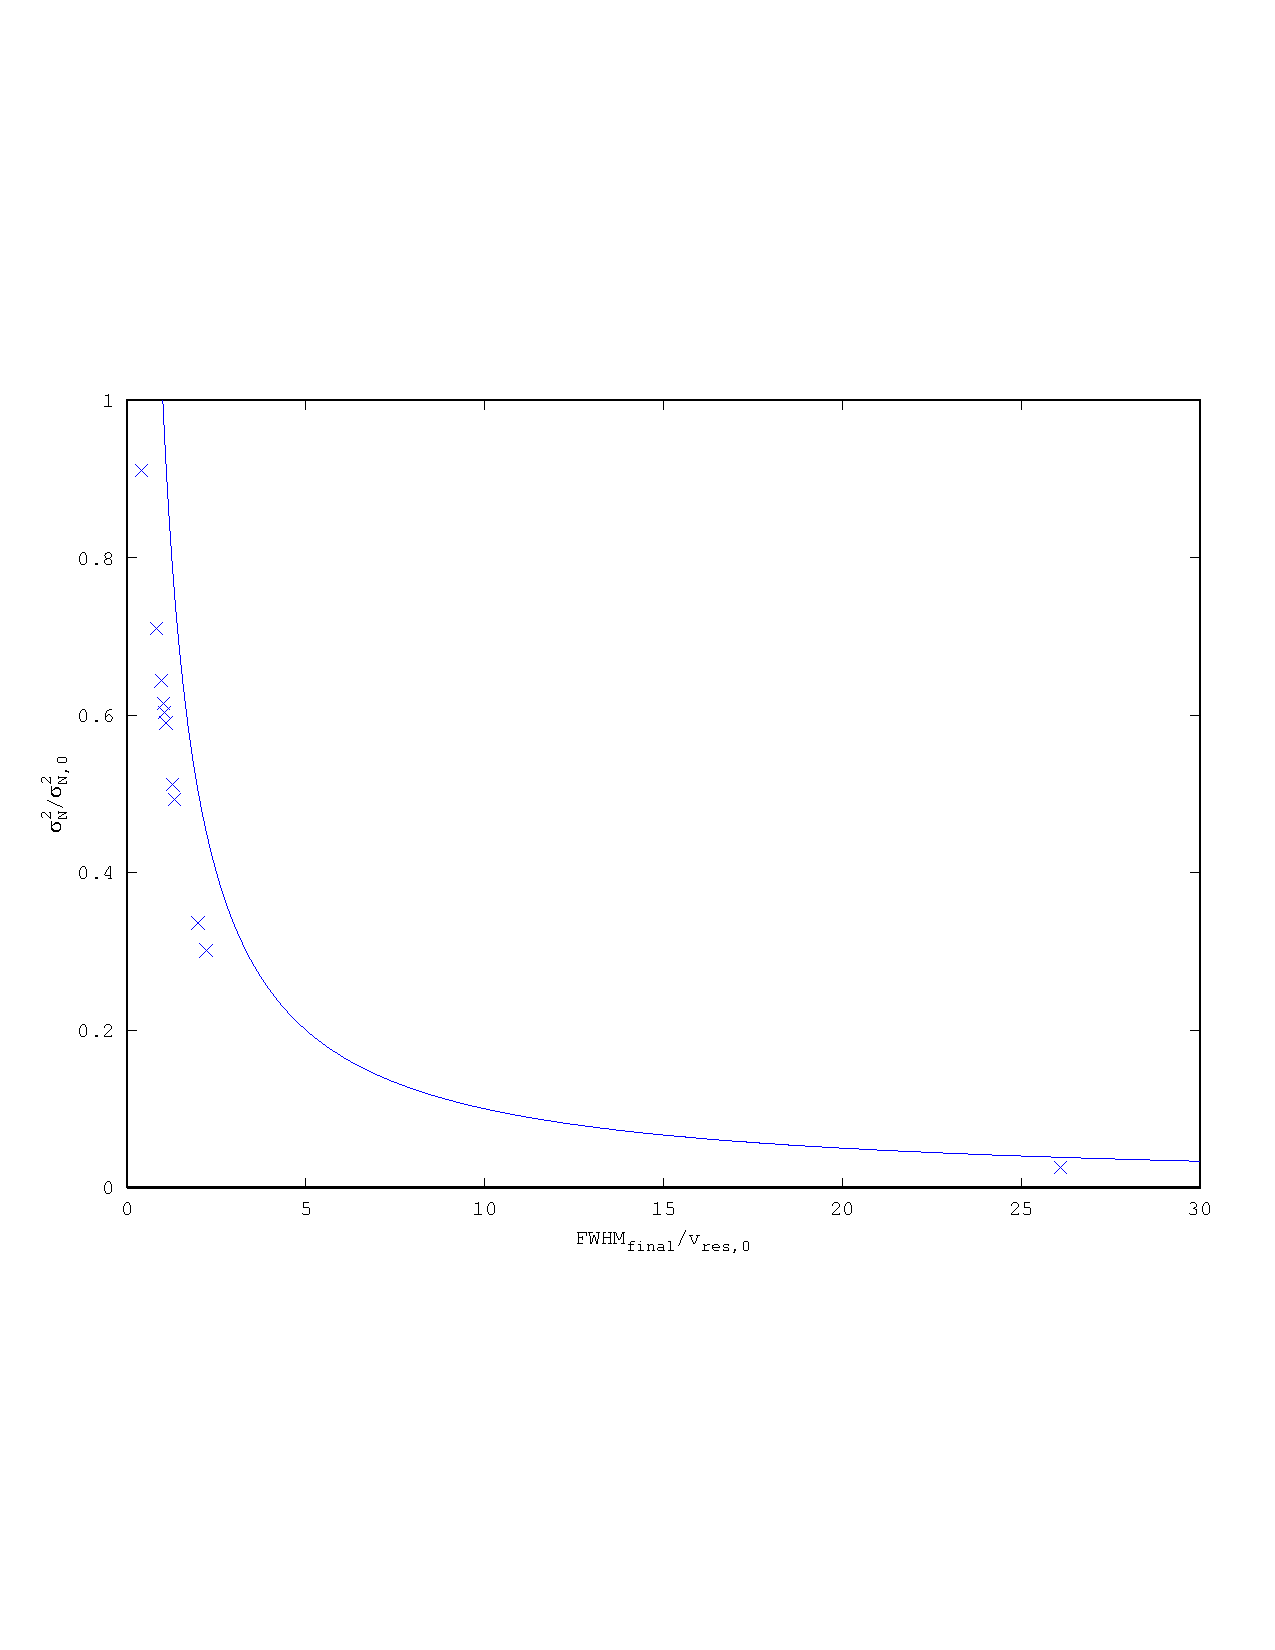
\includegraphics[width=14cm]{NoisePlot.png}
  \caption{The above figure shows the ratio of the smoothed noise variance to the unsmoothed noise variance as a function of the ratio of the original bin width to the FWHM of the Gaussian that we smoothed by. For comparison, we also snow $1/\text{FWHM}$, since the shape of this curve should be similar. }
  \label{fig:todo}
\end{figure}

\begin{figure}[h]
  \centering
  \includegraphics[width=18cm]{CompareTemplates.png}
  \caption{The above figure shows several different quasar continuum composite templates. We have indicated the wavelengths of the \lyb\ line (left), OVI line (middle), and \lya\ line (right). It seems that all templates show emission corresponding to the OVI line.}
  \label{fig:todo}
\end{figure}

\end{document}